\documentclass[11pt,a4paper]{article}

\usepackage[margin=1in]{geometry}
\usepackage{titlesec}
\usepackage{enumitem}
\usepackage{hyperref}
\usepackage{parskip}
\usepackage{graphicx}
\usepackage{float}
\usepackage{booktabs}
\usepackage{amsmath}

\hypersetup{colorlinks=true, linkcolor=blue, urlcolor=blue}

\titleformat{\section}{\large\bfseries}{\thesection}{0.5em}{}
\titleformat{\subsection}{\normalsize\bfseries}{\thesubsection}{0.5em}{}
\setlist{leftmargin=1.4em, topsep=2pt, itemsep=2pt}

\title{\vspace{-1.5cm}\textbf{PKCERT AI \& Software Development Internship \\ Task 08: Classification Models}}
\author{Abdullah Amir}
\date{AI and Software Development \\ 13 July 2026}

\begin{document}

\maketitle
\vspace{-0.8cm}

This report covers the theory and the results. The full code, outputs, and plots
live in the notebook \texttt{classification\_models.ipynb}. The dataset is the
\textbf{Pima Indians Diabetes} set: 768 patients described by 8 clinical
measurements (glucose, BMI, age, and so on), where the goal is to predict whether
a patient has diabetes. About 35 percent of the patients are diabetic, so the
classes are imbalanced, which is exactly why accuracy on its own will not be
enough. A quirk worth flagging up front: several columns use 0 to mean ``not
recorded'', and since a glucose or BMI of zero is physiologically impossible, we
treat those zeros as missing and fill them with the column median before training.

% ----------------------------------------------------------------
\section*{Part A: Logistic Regression}

\textbf{Working principle.} Logistic Regression is a linear model for
classification. It takes a weighted sum of the features, exactly like linear
regression, and then squashes that number through the \textbf{sigmoid} function
\[ \sigma(z) = \frac{1}{1 + e^{-z}}, \qquad z = w_1 x_1 + w_2 x_2 + \dots + w_n x_n + b \]
which maps any real value into the range 0 to 1 and is read as the probability of
the positive class. If that probability is above 0.5 we predict diabetes,
otherwise we predict no diabetes. The weights are learned by maximising the
likelihood of the observed labels, which is the same as minimising the log-loss,
using an iterative solver. Because the model is linear in the features, the sign
and size of each weight tell you how each measurement pushes the predicted risk up
or down, so the model is easy to interpret.

\textbf{Real-world application.} It is the standard tool for medical risk scoring
and credit decisions: estimating a patient's probability of a disease, whether a
transaction is fraudulent, or whether a customer is about to churn. In all of
these you want a calibrated probability and a model you can actually explain to a
doctor or a regulator, and Logistic Regression gives you both.

\textbf{Setup.} We split the data 80/20 with stratification, so both the training
and test sets keep the same 35 percent diabetic ratio, and we standardise the
features. Standardising matters here because the columns live on very different
scales (insulin runs into the hundreds while the pedigree score sits around 0.5),
and the solver converges faster and fairer when everything is on a common scale.
The tree models later do not need this step.

% ----------------------------------------------------------------
\section*{Part B: Classification Metrics}

Accuracy on its own is misleading with imbalanced classes. A lazy model that
always guessed ``no diabetes'' would already score 65 percent here without
learning anything, so we look at the full set of metrics. All four are built from
the four cells of the confusion matrix: true negatives (TN), false positives (FP),
false negatives (FN), and true positives (TP).

\begin{itemize}
    \item \textbf{Accuracy} $=(TP+TN)/\text{all}$. The overall share of correct
    predictions. A good headline number, but blind to \emph{which} class is being
    missed.
    \item \textbf{Precision} $=TP/(TP+FP)$. Of the patients we flagged as
    diabetic, how many really were. High precision means few false alarms.
    \item \textbf{Recall} (sensitivity) $=TP/(TP+FN)$. Of the patients who really
    had diabetes, how many we caught. This is the metric that matters most in
    medical screening, because a false negative, telling a sick patient they are
    healthy, is the costliest error.
    \item \textbf{F1-score} $=2PR/(P+R)$, the harmonic mean of precision and
    recall. One number that stays low unless \emph{both} are high, so it is the
    honest summary when you care about both at once.
\end{itemize}

For the Logistic Regression model the scores on the test set were accuracy
\textbf{0.708}, precision 0.600, recall 0.500, and F1 0.545, with a ROC-AUC of
0.813. The confusion matrix below shows the split of mistakes: 18 false alarms and
27 missed diabetics. That low recall is the model's weak spot at the default 0.5
threshold, and it is the sort of thing you would tune in a real screening setting.

\begin{figure}[H]
    \centering
    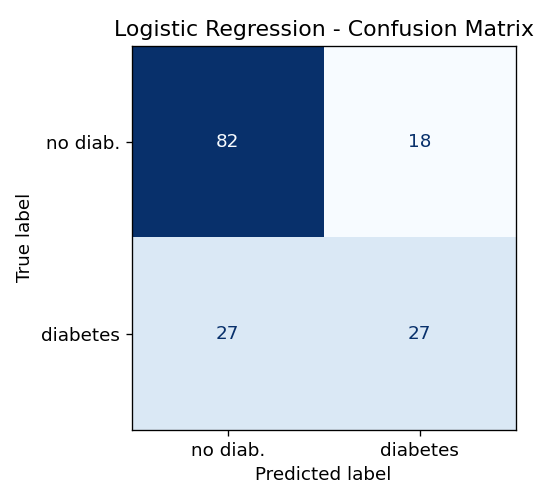
\includegraphics[width=0.46\textwidth]{figures/01_confusion_logreg.png}
    \caption{Logistic Regression confusion matrix. Rows are the true class,
    columns the prediction. The bottom-left cell (27 missed diabetics) is the
    error we most want to reduce.}
\end{figure}

% ----------------------------------------------------------------
\section*{Part C: Decision Trees \& Random Forests}

\textbf{Decision Tree.} A tree asks a sequence of yes/no questions on the features
(``is glucose above 128?'') and follows the branches down to a leaf that holds the
predicted class. At each split it picks the feature and threshold that best
separate the classes, measured by \textbf{Gini impurity} or entropy. Trees need no
feature scaling, they capture non-linear boundaries, and they are wonderfully easy
to read, but a fully grown tree memorises the training data and overfits. We cap
the depth at 4 to keep it honest and legible.

\begin{figure}[H]
    \centering
    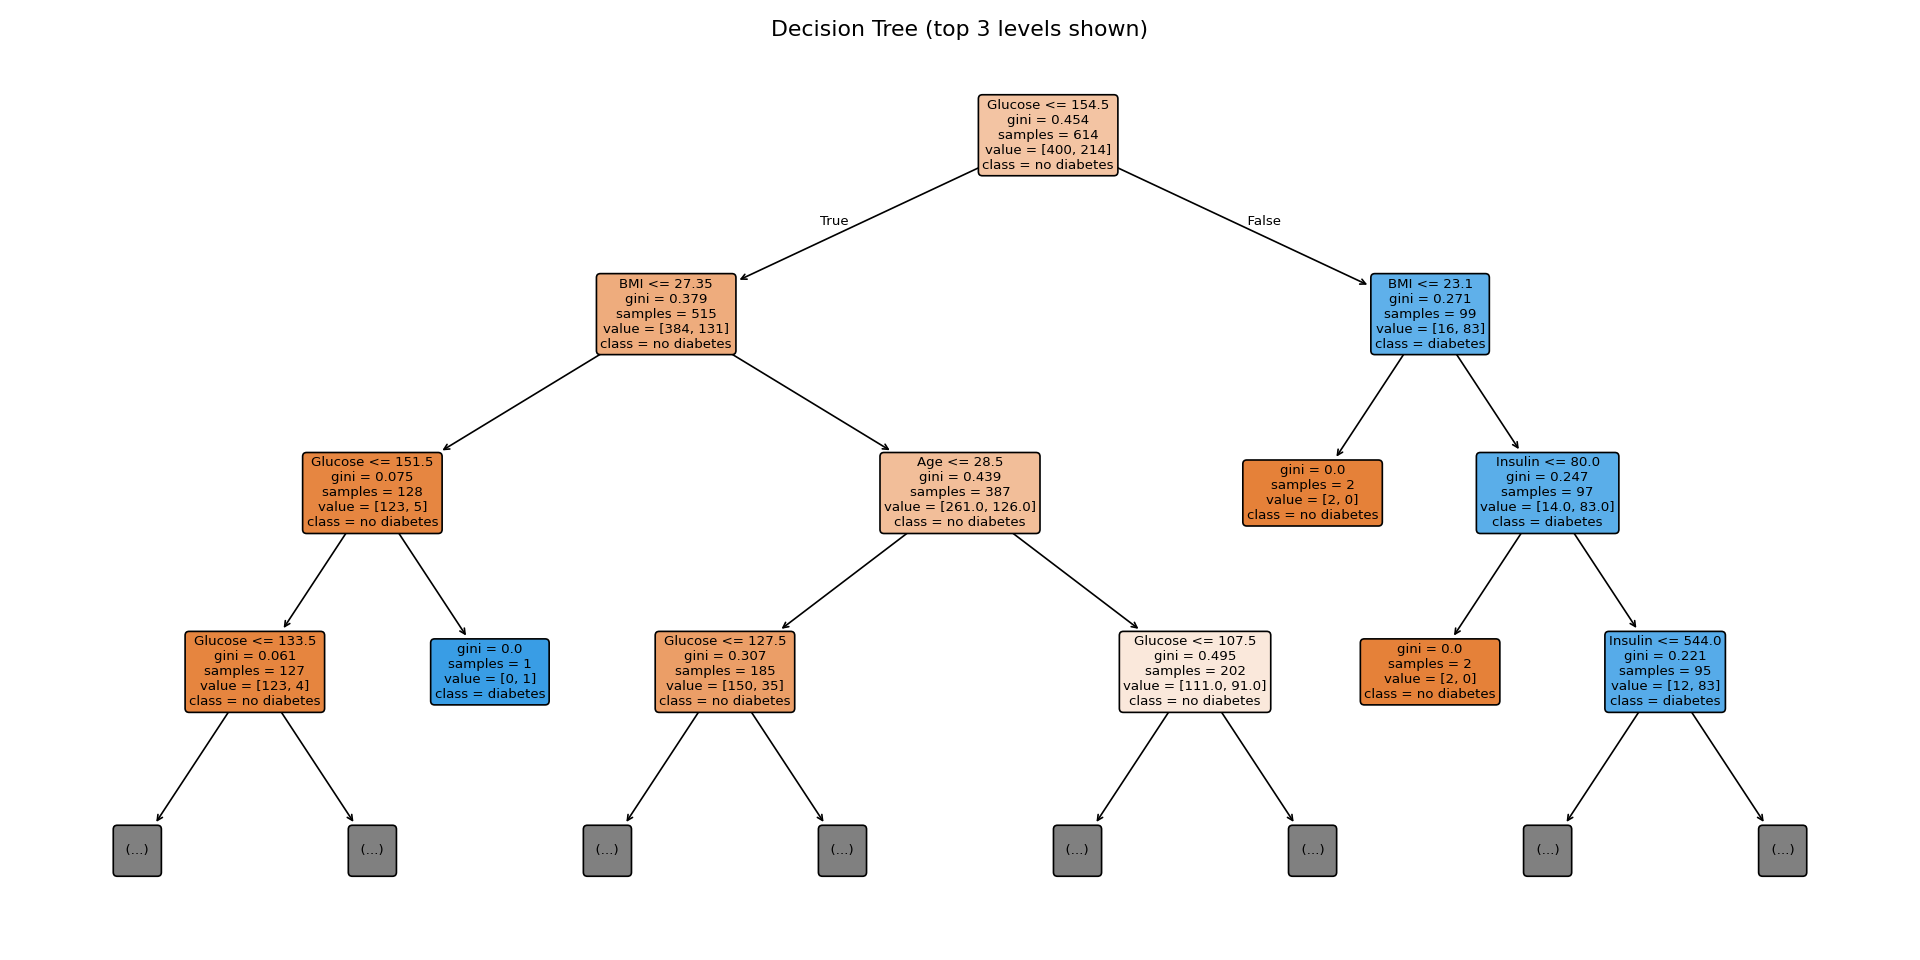
\includegraphics[width=0.92\textwidth]{figures/03_decision_tree.png}
    \caption{The top three levels of the depth-4 tree. Glucose is the very first
    split, which matches the clinical intuition.}
\end{figure}

\textbf{Random Forest.} A forest is an \textbf{ensemble} of many decision trees.
Each tree is trained on a bootstrap sample of the rows and, at every split, may
only look at a random subset of the features. The trees therefore make different
mistakes, and averaging their votes cancels out much of the noise. This
\emph{bagging} keeps most of a single tree's flexibility while sharply cutting the
variance that makes one tree so fragile.

\textbf{Comparison.} On this particular test split the Decision Tree actually came
out ahead of both other models, with accuracy 0.786 and F1 0.692, while the Random
Forest scored accuracy 0.740 and F1 0.600. Taken at face value that looks like a
clear win for the single tree, but the cross-validation in Part D tells a very
different and more trustworthy story. The confusion matrices below and the feature
importances (glucose first, then BMI, family history, and age) round out the
picture.

\begin{figure}[H]
    \centering
    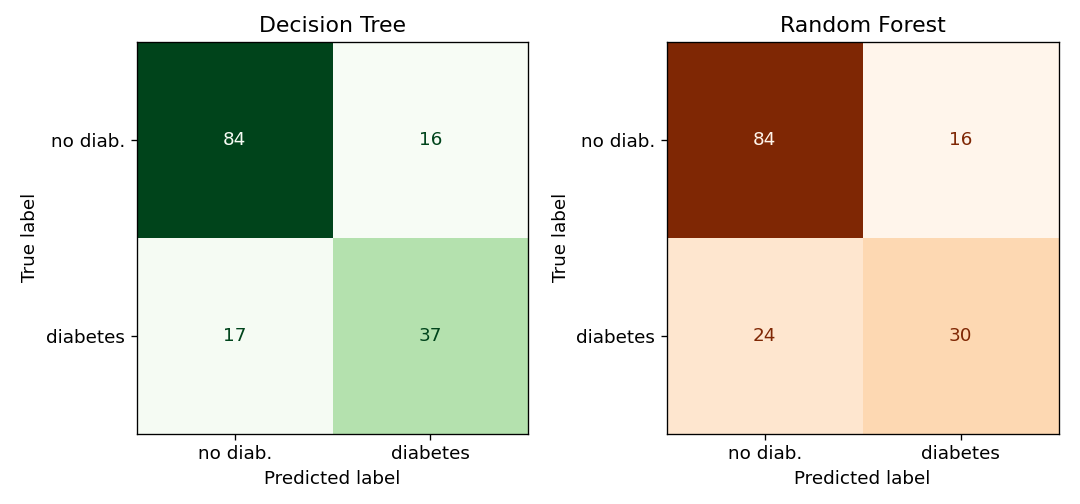
\includegraphics[width=0.62\textwidth]{figures/04_confusion_dt_rf.png}
    \hfill
    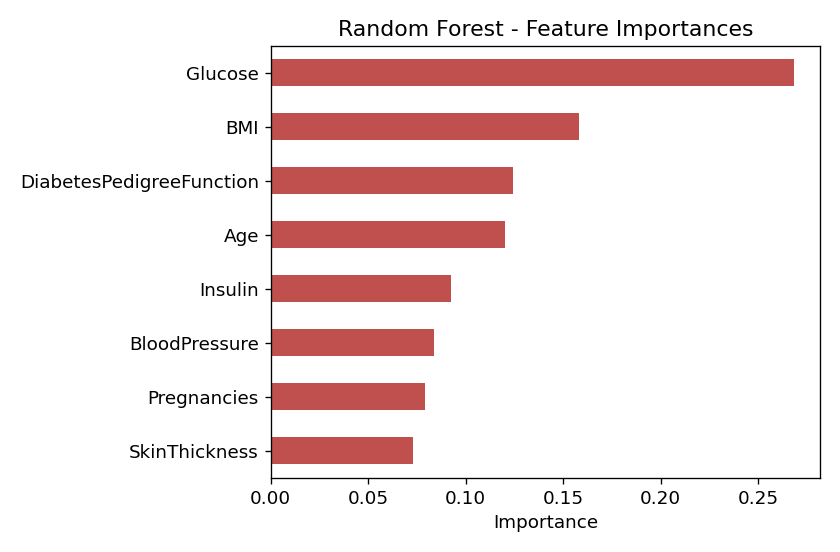
\includegraphics[width=0.36\textwidth]{figures/05_feature_importance.png}
    \caption{Left: confusion matrices for the tree and the forest. Right: the
    forest's feature importances, led by glucose and BMI.}
\end{figure}

\textbf{Advantages and limitations.} A single tree is fast, needs no scaling, and
is fully transparent, but it is high-variance and overfits easily. A forest fixes
the variance problem and is usually more accurate and far more stable, at the cost
of interpretability (it is now 200 trees averaged together) and a bit more compute.

% ----------------------------------------------------------------
\section*{Part D: Comparative Analysis}

Putting all three side by side on the same test set, and then backing it up with
5-fold cross-validation and ROC-AUC, gives a fuller read than any single number.

\begin{table}[H]
\centering
\begin{tabular}{lrrrrrr}
\toprule
\textbf{Model} & \textbf{Accuracy} & \textbf{Precision} & \textbf{Recall} & \textbf{F1} & \textbf{ROC-AUC} & \textbf{CV acc (std)} \\
\midrule
Logistic Regression & 0.708 & 0.600 & 0.500 & 0.545 & 0.813 & 0.772 (0.018) \\
Decision Tree       & 0.786 & 0.698 & 0.685 & 0.692 & 0.789 & 0.732 (0.040) \\
Random Forest       & 0.740 & 0.652 & 0.556 & 0.600 & 0.816 & 0.761 (0.035) \\
\bottomrule
\end{tabular}
\caption{Test-set metrics plus 5-fold cross-validation accuracy. The tree wins the
single split but has the lowest, wobbliest cross-validation score.}
\end{table}

\begin{figure}[H]
    \centering
    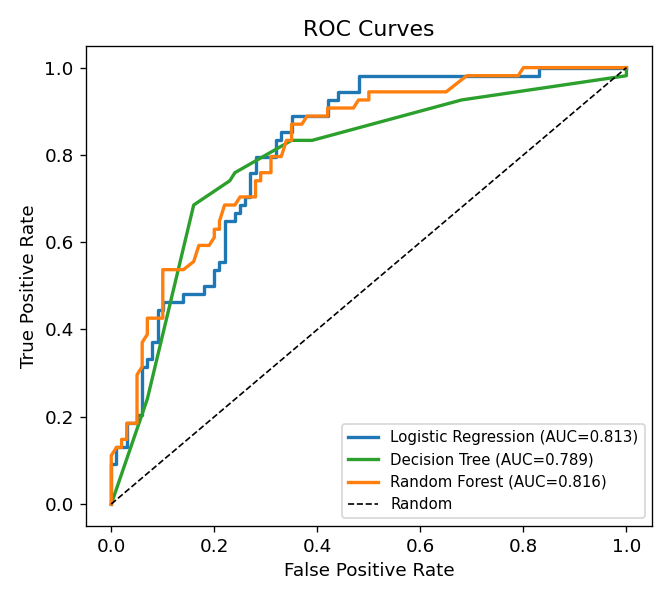
\includegraphics[width=0.44\textwidth]{figures/06_roc_curves.png}
    \hfill
    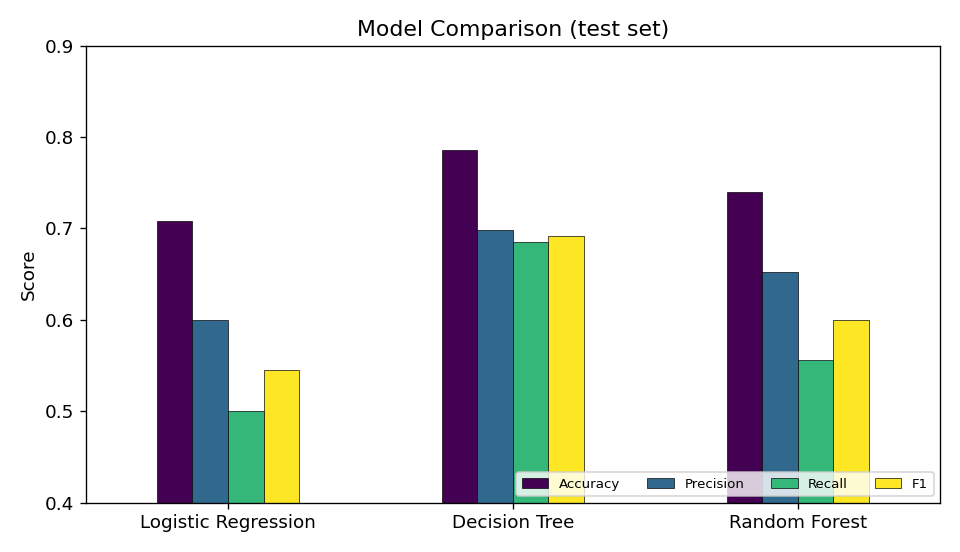
\includegraphics[width=0.52\textwidth]{figures/07_model_comparison.png}
    \caption{Left: ROC curves, where the forest and Logistic Regression edge ahead.
    Right: the four headline metrics side by side.}
\end{figure}

\textbf{Reading the table.} The Decision Tree looks like the winner on this one
split, but cross-validation exposes it as the least reliable of the three: its
average accuracy across five folds is the lowest at 0.732, and its spread is the
widest at 0.040, roughly double the others. That strong test score is mostly luck
of the split. Logistic Regression has the best and steadiest cross-validation
accuracy (0.772, std 0.018) and a near-top ROC-AUC, but its recall at the default
threshold is weak. The Random Forest posts the best ROC-AUC (0.816), the
second-best cross-validation accuracy, and far more stability than the lone tree.

\textbf{Recommendation.} \emph{For this dataset I recommend the Random Forest.}
ROC-AUC measures how well a model ranks patients by risk regardless of where you
put the cut-off, and the forest ranks best. That is what counts in a screening
setting, where you would lower the decision threshold to catch more diabetics,
trading a little precision for the recall you actually care about. The forest is
also far more robust than the single Decision Tree, whose flattering test score
does not survive cross-validation. Logistic Regression is a very strong and more
interpretable runner-up, and would be my pick if a transparent, explainable risk
score mattered more than squeezing out the last bit of ranking accuracy. The lone
Decision Tree is best kept for when a fully readable decision path is the priority.

\vspace{0.4cm}
The notebook and README are on GitHub:
\url{https://github.com/AbdullahAmir06/ai-internship-abdullahamir}.

\end{document}
